% $Id: Component_desdoc.tex,v 1.2 2003/01/21 18:17:03 flanigan Exp $
%
% Earth System Modeling Framework
% Copyright 2002-2003, University Corporation for Atmospheric Research, 
% Massachusetts Institute of Technology, Geophysical Fluid Dynamics 
% Laboratory, University of Michigan, National Centers for Environmental 
% Prediction, Los Alamos National Laboratory, Argonne National Laboratory, 
% NASA Goddard Space Flight Center.
% Licensed under the GPL.


\documentclass[]{article}

\usepackage{epsf}
\usepackage{html}
\usepackage{times}
\usepackage[T1]{fontenc}
\usepackage[dvips]{graphics,color}

\textwidth 6.5in
\textheight 8.5in
\addtolength{\oddsidemargin}{-.75in}
\newcommand{\mytitle}{Component Design Document}
\newcommand{\myauthors}{<Authors>}



\begin{document}


\bodytext{BGCOLOR=white LINK=#083194 VLINK=#21004A}


% Title page
% $Id: title_alldoc.tex,v 1.14 2012/01/06 20:15:12 svasquez Exp $
%
% Earth System Modeling Framework
% Copyright 2002-2013, University Corporation for Atmospheric Research, 
% Massachusetts Institute of Technology, Geophysical Fluid Dynamics 
% Laboratory, University of Michigan, National Centers for Environmental 
% Prediction, Los Alamos National Laboratory, Argonne National Laboratory, 
% NASA Goddard Space Flight Center.
% Licensed under the University of Illinois-NCSA License.


\begin{titlepage}

\begin{center}
{\Large Earth System Modeling Framework } \\
\vspace{.25in}
{\Large {\bf \mytitle}} \\
\vspace{.75in}
{\large {\it \myauthors}} \\
\vspace{.25in}
{\large {\today}}
\vspace{.25in}
\end{center}

\begin{latexonly}
\vspace{4.5in}
\begin{tabular}{p{5in}p{.9in}}
\hrulefill \\
\noindent {\bf NASA Earth Science Technology Office} \\
\noindent Computational Technologies Project \\
\noindent CAN 00-OES-01 \\
\noindent http://www.earthsystemmodeling.org \\
\end{tabular}
\end{latexonly}

\end{titlepage}
















\newpage
\tableofcontents

\newpage


\section{Synopsis}

% $Id: Component_syn.tex,v 1.5 2003/05/07 19:23:00 cdeluca Exp $
%
% Earth System Modeling Framework
% Copyright 2002-2003, University Corporation for Atmospheric Research, 
% Massachusetts Institute of Technology, Geophysical Fluid Dynamics 
% Laboratory, University of Michigan, National Centers for Environmental 
% Prediction, Los Alamos National Laboratory, Argonne National Laboratory, 
% NASA Goddard Space Flight Center.
% Licensed under the GPL.

%\section{Synopsis}

Component, State, and Transform objects are part of the Superstructure 
layer of the Earth System Modeling Framework (ESMF).  They encapsulate
computational models and the exchange of data between them.
They are designed to meet the requirements as specified in the
\htmladdnormallink{ESMF Requirements Document}{http://www.esmf.ucar.edu/esmf_docs/ESMF_reqdoc}.

A {\bf Component} 
is the highest level object in the ESMF object
hierarchy.  Components consist of user supplied code
which follows certain conventions defined by the ESMF framework. 
Components must provide a set of subroutines which match ESMF
defined interfaces. They must encapsulate
all their input and output data in an ESMF {\tt State} object.  They
must able to interpret an ESMF {\tt Time} object in order
to execute the requested number of model timesteps or time interval
before exchanging data with other Components.

Components are identified as being one or more of the
following subtypes: {\bf Application}, {\bf Gridded}, and {\bf Coupler}.  
An Application Component is the top level component which
contains other Components that cooperate in a computation. 
A Gridded Component
does the actual model computation.  A Coupler Component executes or
arranges the execution of the necessary data transformations between one
or more Gridded Components.


A {\bf State} 
encapsulates the data and sufficient description information
to allow the data computed by one Gridded Component to be
used as input to other Gridded Components.  A Gridded Component has
two states, an {\bf Import State} and an {\bf Export State}.
The Import State encapsulates all data needed as input to the
next timestep run of the Component.  The Export State encapsulates 
all data produced by the Component which is required by another
Component as input.  Data inside states are encapsulated by one 
or more of the following ESMF Objects: Bundles, Fields, or Arrays.
Components must exchange information with other Components
only by passing data through State objects.

A Coupler Component takes a list of State objects consisting of
both Export States and Import States.
The Coupler Component is responsible for transforming data 
so the appropriate Import States can be provided the corresponding
Component or Components.
The framework supplies
methods to do basic transformations which may include regridding,
interpolation, unit conversions, accumulations, averaging,
transformations which conserve specific values.


A {\bf Transform} object encapsulates a user-supplied function
containing the processing operations for coupling to be 
performed on a {\tt State} object.  For Components where it is not
feasible to return to the calling routine each time Coupling is
required, the Transform method can be called from within the
Component to perform the proper data transformations.




%\section{Algorithmic Description}

%% $Id: Component_alg.tex,v 1.1 2003/01/07 21:34:21 nscollins Exp $
%
% Earth System Modeling Framework
% Copyright 2002-2003, University Corporation for Atmospheric Research, 
% Massachusetts Institute of Technology, Geophysical Fluid Dynamics 
% Laboratory, University of Michigan, National Centers for Environmental 
% Prediction, Los Alamos National Laboratory, Argonne National Laboratory, 
% NASA Goddard Space Flight Center.
% Licensed under the GPL.

%\section{Algorithmic Description}

<Description of the continuous and discrete scientific algorithms used
in the software.  May reference rather than describe algorithms explicitly.>






\section{Object Model}

% $Id$
%
% Earth System Modeling Framework
% Copyright 2002-2022, University Corporation for Atmospheric Research, 
% Massachusetts Institute of Technology, Geophysical Fluid Dynamics 
% Laboratory, University of Michigan, National Centers for Environmental 
% Prediction, Los Alamos National Laboratory, Argonne National Laboratory, 
% NASA Goddard Space Flight Center.
% Licensed under the University of Illinois-NCSA License.

%\section{Object Model}

The primary ESMF Objects at the Superstructure level include
{\bf Components}, {\bf States}, and optionally {\bf Transforms}.
Components are further identified as being one of the following
subtypes: {\bf Gridded} or {\bf Coupler}.

\begin{center}

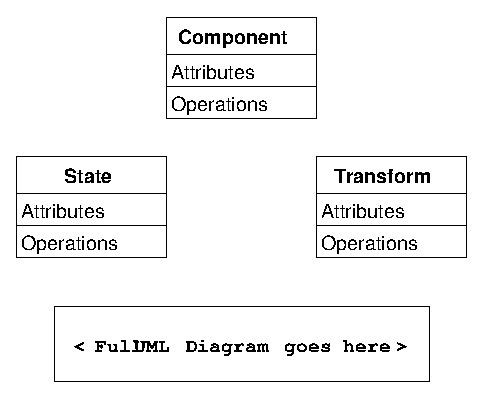
\includegraphics{comp_obj.eps}
   
Figure 1.  Component Class Diagram
   
\end{center}



%\section{Global Parameters and Definitions}
%#ifdef 1 
%\input{Component_param}
%#elif defined(CONSTITUENT)
%\input{comppath/Component_param}
%#endif

%%%%%%%%%%%%% Component Superclass %%%%%%%%%
\section{Component Design}

\subsection{Description}

% $Id: comp_desc.tex,v 1.4 2003/02/20 21:51:59 nscollins Exp $
%
% Earth System Modeling Framework
% Copyright 2002-2003, University Corporation for Atmospheric Research, 
% Massachusetts Institute of Technology, Geophysical Fluid Dynamics 
% Laboratory, University of Michigan, National Centers for Environmental 
% Prediction, Los Alamos National Laboratory, Argonne National Laboratory, 
% NASA Goddard Space Flight Center.
% Licensed under the GPL.

%\subsection{Description}

A {\bf Component}
is the highest level object in the ESMF object
hierarchy.  Components consist of user supplied code
which follows certain conventions defined by the ESMF framework.
Components must provide a set of subroutines which match ESMF
defined interfaces. They must encapsulate
all their input and output data in an ESMF {\tt State} object.  They
must able to interpret an ESMF {\tt Time} object in order
to execute the requested number of model timesteps or time interval
before exchanging data with other Components.

Components are identified as being one or more of the
following subtypes: {\bf Application}, {\bf Gridded}, or {\bf Coupler}.
An Application Component is the top level Component which
contains other Components that cooperate in a computation. 
A Gridded Component
does the actual model computation.  A Coupler Component executes or
arranges the execution of the necessary data transformations between one
or more Gridded Components.





\subsection{Design}

% $Id: comp_design.tex,v 1.2 2003/01/30 23:42:35 nscollins Exp $
%
% Earth System Modeling Framework
% Copyright 2002-2003, University Corporation for Atmospheric Research, 
% Massachusetts Institute of Technology, Geophysical Fluid Dynamics 
% Laboratory, University of Michigan, National Centers for Environmental 
% Prediction, Los Alamos National Laboratory, Argonne National Laboratory, 
% NASA Goddard Space Flight Center.
% Licensed under the GPL.

%\subsection{Design}

The Component class defines a small set of methods (subroutines) which
will be called by higher level code and must be provided by the user.
It uses instances of the State class to identify the data which is
to be exchanged between separate Components.  It uses the Time class
to describe the current model time, timesteps, and time intervals.


There are three subtypes of the Component class.  An Application
Component contains other Component subobjects, and may either be
the main program, or itself a Component nested in a higher level
Application.  A Gridded Component is a computational entity which
consumes and produces data.  A Coupler Component manages the
transformation of data between Components.






\subsubsection{Class Definition}

% $Id: comp_def.tex,v 1.1 2003/01/07 21:34:40 nscollins Exp $
%
% Earth System Modeling Framework
% Copyright 2002-2003, University Corporation for Atmospheric Research, 
% Massachusetts Institute of Technology, Geophysical Fluid Dynamics 
% Laboratory, University of Michigan, National Centers for Environmental 
% Prediction, Los Alamos National Laboratory, Argonne National Laboratory, 
% NASA Goddard Space Flight Center.
% Licensed under the GPL.

%\subsubsection{Class Definition}

<Show internal attributes and methods of derived type, structure or class.

 This definition can be expressed using a general language like UML 
 (see, e.g. ``The Unified Modeling Language Reference Manual,'' 
 Rumbaugh et. al. 1999) or using constructs from a specific language like 
 Fortran.>



\subsubsection{Restrictions}

% $Id: comp_rest.tex,v 1.1 2003/01/07 21:34:46 nscollins Exp $
%
% Earth System Modeling Framework
% Copyright 2002-2003, University Corporation for Atmospheric Research, 
% Massachusetts Institute of Technology, Geophysical Fluid Dynamics 
% Laboratory, University of Michigan, National Centers for Environmental 
% Prediction, Los Alamos National Laboratory, Argonne National Laboratory, 
% NASA Goddard Space Flight Center.
% Licensed under the GPL.

%\subsubsection{Restrictions}

<List class restrictions due to design or implementation strategies.>



\section{Component F90 Interface}

\subsection{Use and Examples}

% $Id: comp_fex.tex,v 1.1 2003/01/07 21:34:45 nscollins Exp $
%
% Earth System Modeling Framework
% Copyright 2002-2003, University Corporation for Atmospheric Research, 
% Massachusetts Institute of Technology, Geophysical Fluid Dynamics 
% Laboratory, University of Michigan, National Centers for Environmental 
% Prediction, Los Alamos National Laboratory, Argonne National Laboratory, 
% NASA Goddard Space Flight Center.
% Licensed under the GPL.

%\subsection{F90 Use and Examples}

<Detailed examples of F90 usage of the class.>



\subsection{Parameters and Definitions}

% $Id: comp_fparam.tex,v 1.1 2003/01/07 21:34:46 nscollins Exp $
%
% Earth System Modeling Framework
% Copyright 2002-2003, University Corporation for Atmospheric Research, 
% Massachusetts Institute of Technology, Geophysical Fluid Dynamics 
% Laboratory, University of Michigan, National Centers for Environmental 
% Prediction, Los Alamos National Laboratory, Argonne National Laboratory, 
% NASA Goddard Space Flight Center.
% Licensed under the GPL.

%\subsection{Parameters}

\begin{description}

\item [<ITEM1>] <Description of ITEM1.>

\item [<ITEM2>] <Description of ITEM2.>

\end{description}











%\subsection{Class API}

\input{comp_fapi}


\section{Component C++ Interface}

\subsection{Use and Examples}

% $ Id: $
%
% Earth System Modeling Framework
% Copyright 2002-2003, University Corporation for Atmospheric Research, 
% Massachusetts Institute of Technology, Geophysical Fluid Dynamics 
% Laboratory, University of Michigan, National Centers for Environmental 
% Prediction, Los Alamos National Laboratory, Argonne National Laboratory, 
% NASA Goddard Space Flight Center.
% Licensed under the GPL.

%\subsection{C++ Use and Examples}

<Detailed examples of C++ usage of the class.>










\subsection{Parameters and Definitions}

% $Id: comp_ccparam.tex,v 1.1 2003/01/07 21:34:40 nscollins Exp $
%
% Earth System Modeling Framework
% Copyright 2002-2003, University Corporation for Atmospheric Research, 
% Massachusetts Institute of Technology, Geophysical Fluid Dynamics 
% Laboratory, University of Michigan, National Centers for Environmental 
% Prediction, Los Alamos National Laboratory, Argonne National Laboratory, 
% NASA Goddard Space Flight Center.
% Licensed under the GPL.

%\subsection{Parameters}

\begin{description}

\item [<ITEM1>] <Description of ITEM1.>

\item [<ITEM2>] <Description of ITEM2.>

\end{description}










%\subsection{Class API}

\input{comp_ccapi}



%%%%%%%%%%%%% Application Class %%%%%%%%%
\section{Application Design}

\subsection{Description}

% $Id: app_desc.tex,v 1.2 2003/02/03 17:08:22 nscollins Exp $
%
% Earth System Modeling Framework
% Copyright 2002-2003, University Corporation for Atmospheric Research, 
% Massachusetts Institute of Technology, Geophysical Fluid Dynamics 
% Laboratory, University of Michigan, National Centers for Environmental 
% Prediction, Los Alamos National Laboratory, Argonne National Laboratory, 
% NASA Goddard Space Flight Center.
% Licensed under the GPL.

%\subsection{Description}

< a specialization of the generic Component object.  what's different...>

< include description here about main programs vs applications which
are themselves a component, and the minimal driver layer needed if
the higher level program isn't wanted >



\subsection{Design}

% $Id: app_design.tex,v 1.2 2003/02/20 17:31:23 nscollins Exp $
%
% Earth System Modeling Framework
% Copyright 2002-2003, University Corporation for Atmospheric Research, 
% Massachusetts Institute of Technology, Geophysical Fluid Dynamics 
% Laboratory, University of Michigan, National Centers for Environmental 
% Prediction, Los Alamos National Laboratory, Argonne National Laboratory, 
% NASA Goddard Space Flight Center.
% Licensed under the GPL.

%\subsection{Design}

The Application Component encapsulates the internal state of the
application, including the Layout, the Clock, the subcomponents,
and the State and Transform objects needed to communicate data
between subcomponents.





\subsubsection{Class Definition}

% $Id: app_def.tex,v 1.1 2003/01/07 21:34:31 nscollins Exp $
%
% Earth System Modeling Framework
% Copyright 2002-2003, University Corporation for Atmospheric Research, 
% Massachusetts Institute of Technology, Geophysical Fluid Dynamics 
% Laboratory, University of Michigan, National Centers for Environmental 
% Prediction, Los Alamos National Laboratory, Argonne National Laboratory, 
% NASA Goddard Space Flight Center.
% Licensed under the GPL.

%\subsubsection{Class Definition}

<Show internal attributes and methods of derived type, structure or class.

 This definition can be expressed using a general language like UML 
 (see, e.g. ``The Unified Modeling Language Reference Manual,'' 
 Rumbaugh et. al. 1999) or using constructs from a specific language like 
 Fortran.>



\subsubsection{Restrictions}

% $Id: app_rest.tex,v 1.2 2003/02/20 17:31:23 nscollins Exp $
%
% Earth System Modeling Framework
% Copyright 2002-2003, University Corporation for Atmospheric Research, 
% Massachusetts Institute of Technology, Geophysical Fluid Dynamics 
% Laboratory, University of Michigan, National Centers for Environmental 
% Prediction, Los Alamos National Laboratory, Argonne National Laboratory, 
% NASA Goddard Space Flight Center.
% Licensed under the GPL.

%\subsubsection{Restrictions}

An Application which is written as a main program cannot
be embedded in a higher level application.




\section{Application F90 Interface}

\subsection{Use and Examples}

% $Id: app_fex.tex,v 1.1 2003/01/07 21:34:35 nscollins Exp $
%
% Earth System Modeling Framework
% Copyright 2002-2003, University Corporation for Atmospheric Research, 
% Massachusetts Institute of Technology, Geophysical Fluid Dynamics 
% Laboratory, University of Michigan, National Centers for Environmental 
% Prediction, Los Alamos National Laboratory, Argonne National Laboratory, 
% NASA Goddard Space Flight Center.
% Licensed under the GPL.

%\subsection{F90 Use and Examples}

<Detailed examples of F90 usage of the class.>



\subsection{Parameters and Definitions}

% $Id: app_fparam.tex,v 1.1 2003/01/07 21:34:36 nscollins Exp $
%
% Earth System Modeling Framework
% Copyright 2002-2003, University Corporation for Atmospheric Research, 
% Massachusetts Institute of Technology, Geophysical Fluid Dynamics 
% Laboratory, University of Michigan, National Centers for Environmental 
% Prediction, Los Alamos National Laboratory, Argonne National Laboratory, 
% NASA Goddard Space Flight Center.
% Licensed under the GPL.

%\subsection{Parameters}

\begin{description}

\item [<ITEM1>] <Description of ITEM1.>

\item [<ITEM2>] <Description of ITEM2.>

\end{description}











%\subsection{Class API}

\input{app_fapi}


\section{Application C++ Interface}

\subsection{Use and Examples}

% $ Id: $
%
% Earth System Modeling Framework
% Copyright 2002-2003, University Corporation for Atmospheric Research, 
% Massachusetts Institute of Technology, Geophysical Fluid Dynamics 
% Laboratory, University of Michigan, National Centers for Environmental 
% Prediction, Los Alamos National Laboratory, Argonne National Laboratory, 
% NASA Goddard Space Flight Center.
% Licensed under the GPL.

%\subsection{C++ Use and Examples}

<Detailed examples of C++ usage of the class.>










\subsection{Parameters and Definitions}

% $Id: app_ccparam.tex,v 1.1 2003/01/07 21:34:31 nscollins Exp $
%
% Earth System Modeling Framework
% Copyright 2002-2003, University Corporation for Atmospheric Research, 
% Massachusetts Institute of Technology, Geophysical Fluid Dynamics 
% Laboratory, University of Michigan, National Centers for Environmental 
% Prediction, Los Alamos National Laboratory, Argonne National Laboratory, 
% NASA Goddard Space Flight Center.
% Licensed under the GPL.

%\subsection{Parameters}

\begin{description}

\item [<ITEM1>] <Description of ITEM1.>

\item [<ITEM2>] <Description of ITEM2.>

\end{description}










%\subsection{Class API}

\input{app_ccapi}





%%%%%%%%%%%%% Coupler Class %%%%%%%%%
\section{Coupler Design}

\subsection{Description}

% $Id: cpl_desc.tex,v 1.1 2003/01/07 21:34:52 nscollins Exp $
%
% Earth System Modeling Framework
% Copyright 2002-2003, University Corporation for Atmospheric Research, 
% Massachusetts Institute of Technology, Geophysical Fluid Dynamics 
% Laboratory, University of Michigan, National Centers for Environmental 
% Prediction, Los Alamos National Laboratory, Argonne National Laboratory, 
% NASA Goddard Space Flight Center.
% Licensed under the GPL.

%\subsection{Description}

<Describe class function and relation to other classes.>



\subsection{Design}

% $Id: cpl_design.tex,v 1.1 2003/01/07 21:34:53 nscollins Exp $
%
% Earth System Modeling Framework
% Copyright 2002-2003, University Corporation for Atmospheric Research, 
% Massachusetts Institute of Technology, Geophysical Fluid Dynamics 
% Laboratory, University of Michigan, National Centers for Environmental 
% Prediction, Los Alamos National Laboratory, Argonne National Laboratory, 
% NASA Goddard Space Flight Center.
% Licensed under the GPL.

%\subsection{Design}

<Describe strategy for overall class design.>






\subsubsection{Class Definition}

% $Id: cpl_def.tex,v 1.1 2003/01/07 21:34:52 nscollins Exp $
%
% Earth System Modeling Framework
% Copyright 2002-2003, University Corporation for Atmospheric Research, 
% Massachusetts Institute of Technology, Geophysical Fluid Dynamics 
% Laboratory, University of Michigan, National Centers for Environmental 
% Prediction, Los Alamos National Laboratory, Argonne National Laboratory, 
% NASA Goddard Space Flight Center.
% Licensed under the GPL.

%\subsubsection{Class Definition}

<Show internal attributes and methods of derived type, structure or class.

 This definition can be expressed using a general language like UML 
 (see, e.g. ``The Unified Modeling Language Reference Manual,'' 
 Rumbaugh et. al. 1999) or using constructs from a specific language like 
 Fortran.>



\subsubsection{Restrictions}

% $Id: cpl_rest.tex,v 1.2 2003/02/20 17:31:24 nscollins Exp $
%
% Earth System Modeling Framework
% Copyright 2002-2003, University Corporation for Atmospheric Research, 
% Massachusetts Institute of Technology, Geophysical Fluid Dynamics 
% Laboratory, University of Michigan, National Centers for Environmental 
% Prediction, Los Alamos National Laboratory, Argonne National Laboratory, 
% NASA Goddard Space Flight Center.
% Licensed under the GPL.

%\subsubsection{Restrictions}

Couplers are user-written code and need to be
customized for each combination of Components
which they are interacting with.




\section{Coupler F90 Interface}

\subsection{Use and Examples}

% $Id: cpl_fex.tex,v 1.1 2003/01/07 21:34:57 nscollins Exp $
%
% Earth System Modeling Framework
% Copyright 2002-2003, University Corporation for Atmospheric Research, 
% Massachusetts Institute of Technology, Geophysical Fluid Dynamics 
% Laboratory, University of Michigan, National Centers for Environmental 
% Prediction, Los Alamos National Laboratory, Argonne National Laboratory, 
% NASA Goddard Space Flight Center.
% Licensed under the GPL.

%\subsection{F90 Use and Examples}

<Detailed examples of F90 usage of the class.>



\subsection{Parameters and Definitions}

% $Id: cpl_fparam.tex,v 1.1 2003/01/07 21:34:57 nscollins Exp $
%
% Earth System Modeling Framework
% Copyright 2002-2003, University Corporation for Atmospheric Research, 
% Massachusetts Institute of Technology, Geophysical Fluid Dynamics 
% Laboratory, University of Michigan, National Centers for Environmental 
% Prediction, Los Alamos National Laboratory, Argonne National Laboratory, 
% NASA Goddard Space Flight Center.
% Licensed under the GPL.

%\subsection{Parameters}

\begin{description}

\item [<ITEM1>] <Description of ITEM1.>

\item [<ITEM2>] <Description of ITEM2.>

\end{description}











%\subsection{Class API}

\input{cpl_fapi}


\section{Coupler C++ Interface}

\subsection{Use and Examples}

% $ Id: $
%
% Earth System Modeling Framework
% Copyright 2002-2003, University Corporation for Atmospheric Research, 
% Massachusetts Institute of Technology, Geophysical Fluid Dynamics 
% Laboratory, University of Michigan, National Centers for Environmental 
% Prediction, Los Alamos National Laboratory, Argonne National Laboratory, 
% NASA Goddard Space Flight Center.
% Licensed under the GPL.

%\subsection{C++ Use and Examples}

<Detailed examples of C++ usage of the class.>










\subsection{Parameters and Definitions}

% $Id: cpl_ccparam.tex,v 1.1 2003/01/07 21:34:51 nscollins Exp $
%
% Earth System Modeling Framework
% Copyright 2002-2003, University Corporation for Atmospheric Research, 
% Massachusetts Institute of Technology, Geophysical Fluid Dynamics 
% Laboratory, University of Michigan, National Centers for Environmental 
% Prediction, Los Alamos National Laboratory, Argonne National Laboratory, 
% NASA Goddard Space Flight Center.
% Licensed under the GPL.

%\subsection{Parameters}

\begin{description}

\item [<ITEM1>] <Description of ITEM1.>

\item [<ITEM2>] <Description of ITEM2.>

\end{description}










%\subsection{Class API}

\input{cpl_ccapi}





%%%%%%%%%%%%% Gridded Component Class %%%%%%%%%
\section{Gridded Component Design}

\subsection{Description}

% $Id: gcomp_desc.tex,v 1.2 2003/02/03 17:08:24 nscollins Exp $
%
% Earth System Modeling Framework
% Copyright 2002-2003, University Corporation for Atmospheric Research, 
% Massachusetts Institute of Technology, Geophysical Fluid Dynamics 
% Laboratory, University of Michigan, National Centers for Environmental 
% Prediction, Los Alamos National Laboratory, Argonne National Laboratory, 
% NASA Goddard Space Flight Center.
% Licensed under the GPL.

%\subsection{Description}

< a specialization of the generic Component object.  what's different...>

< conceptually simplest is a sequential component, which 
takes an import state, runs the requested time, and produces
an export state.  also possible are concurrent components
which take a transform as input, and then run until the stop
time.  when communication is needed, the transform routine
is called. all data goes thru states. >



\subsection{Design}

% $Id: gcomp_design.tex,v 1.1 2003/01/07 21:35:06 nscollins Exp $
%
% Earth System Modeling Framework
% Copyright 2002-2003, University Corporation for Atmospheric Research, 
% Massachusetts Institute of Technology, Geophysical Fluid Dynamics 
% Laboratory, University of Michigan, National Centers for Environmental 
% Prediction, Los Alamos National Laboratory, Argonne National Laboratory, 
% NASA Goddard Space Flight Center.
% Licensed under the GPL.

%\subsection{Design}

<Describe strategy for overall class design.>






\subsubsection{Class Definition}

% $Id: gcomp_def.tex,v 1.1 2003/01/07 21:35:00 nscollins Exp $
%
% Earth System Modeling Framework
% Copyright 2002-2003, University Corporation for Atmospheric Research, 
% Massachusetts Institute of Technology, Geophysical Fluid Dynamics 
% Laboratory, University of Michigan, National Centers for Environmental 
% Prediction, Los Alamos National Laboratory, Argonne National Laboratory, 
% NASA Goddard Space Flight Center.
% Licensed under the GPL.

%\subsubsection{Class Definition}

<Show internal attributes and methods of derived type, structure or class.

 This definition can be expressed using a general language like UML 
 (see, e.g. ``The Unified Modeling Language Reference Manual,'' 
 Rumbaugh et. al. 1999) or using constructs from a specific language like 
 Fortran.>



\subsubsection{Restrictions}

% $Id: gcomp_rest.tex,v 1.3 2004/03/22 19:18:03 cdeluca Exp $
%
% Earth System Modeling Framework
% Copyright 2002-2003, University Corporation for Atmospheric Research, 
% Massachusetts Institute of Technology, Geophysical Fluid Dynamics 
% Laboratory, University of Michigan, National Centers for Environmental 
% Prediction, Los Alamos National Laboratory, Argonne National Laboratory, 
% NASA Goddard Space Flight Center.
% Licensed under the GPL.

%\subsubsection{Restrictions and Future Work}

Gridded Components must only communicate with other
Components via data in State objects.  They must 
not make direct references to data in other states.

If possible, Components should attempt to make all
data private, so public names do not interfere with data in
other components.




\section{Gridded Component F90 Interface}

\subsection{Use and Examples}

% $Id: gcomp_fex.tex,v 1.1 2003/01/07 21:35:09 nscollins Exp $
%
% Earth System Modeling Framework
% Copyright 2002-2003, University Corporation for Atmospheric Research, 
% Massachusetts Institute of Technology, Geophysical Fluid Dynamics 
% Laboratory, University of Michigan, National Centers for Environmental 
% Prediction, Los Alamos National Laboratory, Argonne National Laboratory, 
% NASA Goddard Space Flight Center.
% Licensed under the GPL.

%\subsection{F90 Use and Examples}

<Detailed examples of F90 usage of the class.>



\subsection{Parameters and Definitions}

% $Id: gcomp_fparam.tex,v 1.1 2003/01/07 21:35:14 nscollins Exp $
%
% Earth System Modeling Framework
% Copyright 2002-2003, University Corporation for Atmospheric Research, 
% Massachusetts Institute of Technology, Geophysical Fluid Dynamics 
% Laboratory, University of Michigan, National Centers for Environmental 
% Prediction, Los Alamos National Laboratory, Argonne National Laboratory, 
% NASA Goddard Space Flight Center.
% Licensed under the GPL.

%\subsection{Parameters}

\begin{description}

\item [<ITEM1>] <Description of ITEM1.>

\item [<ITEM2>] <Description of ITEM2.>

\end{description}











%\subsection{Class API}

\input{gcomp_fapi}


\section{Gridded Component C++ Interface}

\subsection{Use and Examples}

% $ Id: $
%
% Earth System Modeling Framework
% Copyright 2002-2003, University Corporation for Atmospheric Research, 
% Massachusetts Institute of Technology, Geophysical Fluid Dynamics 
% Laboratory, University of Michigan, National Centers for Environmental 
% Prediction, Los Alamos National Laboratory, Argonne National Laboratory, 
% NASA Goddard Space Flight Center.
% Licensed under the GPL.

%\subsection{C++ Use and Examples}

<Detailed examples of C++ usage of the class.>










\subsection{Parameters and Definitions}

% $Id: gcomp_ccparam.tex,v 1.1 2003/01/07 21:34:59 nscollins Exp $
%
% Earth System Modeling Framework
% Copyright 2002-2003, University Corporation for Atmospheric Research, 
% Massachusetts Institute of Technology, Geophysical Fluid Dynamics 
% Laboratory, University of Michigan, National Centers for Environmental 
% Prediction, Los Alamos National Laboratory, Argonne National Laboratory, 
% NASA Goddard Space Flight Center.
% Licensed under the GPL.

%\subsection{Parameters}

\begin{description}

\item [<ITEM1>] <Description of ITEM1.>

\item [<ITEM2>] <Description of ITEM2.>

\end{description}










%\subsection{Class API}

\input{gcomp_ccapi}




%%%%%%%%%%%%% State Class %%%%%%%%%
\section{State Design}

\subsection{Description}

% $Id: state_desc.tex,v 1.2 2003/01/28 23:58:32 nscollins Exp $
%
% Earth System Modeling Framework
% Copyright 2002-2003, University Corporation for Atmospheric Research, 
% Massachusetts Institute of Technology, Geophysical Fluid Dynamics 
% Laboratory, University of Michigan, National Centers for Environmental 
% Prediction, Los Alamos National Laboratory, Argonne National Laboratory, 
% NASA Goddard Space Flight Center.
% Licensed under the GPL.

%\subsection{Description}

A State object contains the data and description information needed to
communicate data between multiple Components.

If a Gridded Component object needs data
from another Component to run it will query its associated
Import State for the data.  If a Gridded Component creates data
needed by another Component it will put that data into an
Export State.  A Coupler Component can read one or more Export States,
operate on the data as required, and can create one or more Import States.

 



\subsection{Design}

% $Id: state_design.tex,v 1.2 2003/01/28 23:58:32 nscollins Exp $
%
% Earth System Modeling Framework
% Copyright 2002-2003, University Corporation for Atmospheric Research, 
% Massachusetts Institute of Technology, Geophysical Fluid Dynamics 
% Laboratory, University of Michigan, National Centers for Environmental 
% Prediction, Los Alamos National Laboratory, Argonne National Laboratory, 
% NASA Goddard Space Flight Center.
% Licensed under the GPL.

%\subsection{Design}

A State object encapsulates all data being communicated into and
out of a Gridded Component explicitly.  No private communication
of data between Components is permitted in order to maintain the
independence of Components and to enable Components to be replaced
without rewriting the internal code inside the Component.

States contain the name of the associated Component, a flag for Import
or Export, and a list of data objects, which can be a combination of
Bundles, Fields, and/or Arrays.  The objects must be named and have
the proper attributes so they can be identified by the receiver of
the data.  For example, units may need to be associated with the data
as an Attribute.  The standard CF naming convention for data 
should be followed.

States can be create and deleted, have data added or deleted from them,
and queried for various kinds of information.

Transform methods operate on States, doing regridding, interpolation,
summation, averaging, transposes, and other operations needed to
make the export State of one Component suitable for import to another
Component.



\subsubsection{Class Definition}

% $Id: state_def.tex,v 1.1 2003/01/07 21:35:23 nscollins Exp $
%
% Earth System Modeling Framework
% Copyright 2002-2003, University Corporation for Atmospheric Research, 
% Massachusetts Institute of Technology, Geophysical Fluid Dynamics 
% Laboratory, University of Michigan, National Centers for Environmental 
% Prediction, Los Alamos National Laboratory, Argonne National Laboratory, 
% NASA Goddard Space Flight Center.
% Licensed under the GPL.

%\subsubsection{Class Definition}

<Show internal attributes and methods of derived type, structure or class.

 This definition can be expressed using a general language like UML 
 (see, e.g. ``The Unified Modeling Language Reference Manual,'' 
 Rumbaugh et. al. 1999) or using constructs from a specific language like 
 Fortran.>



\subsubsection{Restrictions}

% $Id: state_rest.tex,v 1.2 2003/01/28 23:58:32 nscollins Exp $
%
% Earth System Modeling Framework
% Copyright 2002-2003, University Corporation for Atmospheric Research, 
% Massachusetts Institute of Technology, Geophysical Fluid Dynamics 
% Laboratory, University of Michigan, National Centers for Environmental 
% Prediction, Los Alamos National Laboratory, Argonne National Laboratory, 
% NASA Goddard Space Flight Center.
% Licensed under the GPL.

%\subsubsection{Restrictions}

The initial implementation of States will only support Bundles and
Arrays.  Single Fields should be encapsulated in a Bundle before
being added to an Export State.






\section{State F90 Interface}

\subsection{Use and Examples}

% $Id: state_fex.tex,v 1.1 2003/01/07 21:35:28 nscollins Exp $
%
% Earth System Modeling Framework
% Copyright 2002-2003, University Corporation for Atmospheric Research, 
% Massachusetts Institute of Technology, Geophysical Fluid Dynamics 
% Laboratory, University of Michigan, National Centers for Environmental 
% Prediction, Los Alamos National Laboratory, Argonne National Laboratory, 
% NASA Goddard Space Flight Center.
% Licensed under the GPL.

%\subsection{F90 Use and Examples}

<Detailed examples of F90 usage of the class.>



\subsection{Parameters and Definitions}

% $Id: state_fparam.tex,v 1.1 2003/01/07 21:35:33 nscollins Exp $
%
% Earth System Modeling Framework
% Copyright 2002-2003, University Corporation for Atmospheric Research, 
% Massachusetts Institute of Technology, Geophysical Fluid Dynamics 
% Laboratory, University of Michigan, National Centers for Environmental 
% Prediction, Los Alamos National Laboratory, Argonne National Laboratory, 
% NASA Goddard Space Flight Center.
% Licensed under the GPL.

%\subsection{Parameters}

\begin{description}

\item [<ITEM1>] <Description of ITEM1.>

\item [<ITEM2>] <Description of ITEM2.>

\end{description}











%\subsection{Class API}

%                **** IMPORTANT NOTICE *****
% This LaTeX file has been automatically produced by ProTeX v. 1.1
% Any changes made to this file will likely be lost next time
% this file is regenerated from its source. Send questions 
% to Arlindo da Silva, dasilva@gsfc.nasa.gov
 
\parskip        0pt
\parindent      0pt
\baselineskip  11pt
 
%--------------------- SHORT-HAND MACROS ----------------------
\def\bv{\begin{verbatim}}
\def\ev{\end{verbatim}}
\def\be{\begin{equation}}
\def\ee{\end{equation}}
\def\bea{\begin{eqnarray}}
\def\eea{\end{eqnarray}}
\def\bi{\begin{itemize}}
\def\ei{\end{itemize}}
\def\bn{\begin{enumerate}}
\def\en{\end{enumerate}}
\def\bd{\begin{description}}
\def\ed{\end{description}}
\def\({\left (}
\def\){\right )}
\def\[{\left [}
\def\]{\right ]}
\def\<{\left  \langle}
\def\>{\right \rangle}
\def\cI{{\cal I}}
\def\diag{\mathop{\rm diag}}
\def\tr{\mathop{\rm tr}}
%-------------------------------------------------------------

\markboth{Left}{Source File: ESMF\_State.F90,  Date: Tue Jan 28 16:56:54 MST 2003
}

 
%/////////////////////////////////////////////////////////////
\subsection{Fortran:  Module Interface ESMF\_StateMod - Manage data states uniformly between F90 and C++  (Source File: ESMF\_State.F90)}


  
  
   The code in this file implements the Fortran interfaces to the
   {\tt State} class and associated functions and subroutines.  
  
  
  ------------------------------------------------------------------------------
\bigskip{\em USES:}
\begin{verbatim}       use ESMF_BaseMod
       use ESMF_IOMod
       !use ESMF_ComponentMod
       implicit none
 
  ------------------------------------------------------------------------------\end{verbatim}{\sf PRIVATE TYPES:}
\begin{verbatim}       private
 
  ------------------------------------------------------------------------------
       ! ESMF_StateImpExpType
       !   Enumerated value for storing Import or Export State type.
       type ESMF_StateImpExpType
       sequence
       private
          integer :: state
       end type
 
       type(ESMF_StateImpExpType), parameter :: &
                 ESMF_STATEIMPORT = ESMF_StateImpExpType(1), &
                 ESMF_STATEEXPORT = ESMF_StateImpExpType(2), &
                 ESMF_STATEUNKNOWN = ESMF_StateImpExpType(3)
 
  ------------------------------------------------------------------------------
       ! ESMF_StateObjectType
       !   Each entry in the list of states is either simply a name placeholder
       !   or an actual data item - Bundle, Field, or Array.  The state list
       !   can either be a linked list or an array of derived types.
       !   For a linked list, the Last is the end of the list.
       type ESMF_StateObjectType
       sequence
       private
          integer :: ot
       end type
 
       type(ESMF_StateObjectType), parameter :: &
                 ESMF_BUNDLE = ESMF_StateObjectType(1), &
                 ESMF_FIELD = ESMF_StateObjectType(2), &
                 ESMF_ARRAY = ESMF_StateObjectType(3), &
                 ESMF_DATANAME = ESMF_StateObjectType(4), &
                 ESMF_LAST = ESMF_StateObjectType(5), &
                 ESMF_OBJTYPEUNKNOWN = ESMF_StateObjectType(6)
 
  ------------------------------------------------------------------------------
       ! ESMF_StateDataNeeded
       !   For an Export State if all data which can potentially be created is
       !   not needed, this flag can be used to mark data which does not need
       !   to be created by the Component.
       type ESMF_StateDataNeeded
       sequence
       private
          integer :: needed
       end type
 
       type(ESMF_StateDataNeeded), parameter :: &
                 ESMF_NEEDED = ESMF_StateDataNeeded(1), &
                 ESMF_NOTNEEDED= ESMF_StateDataNeeded(2), &
                 ESMF_DONOTCARE = ESMF_StateDataNeeded(3), &
                 ESMF_NEEDUNKNOWN = ESMF_StateDataNeeded(4)
 
  ------------------------------------------------------------------------------
       ! ESMF_StateDataReady
       type ESMF_StateDataReady
       sequence
       private
          integer :: ready
       end type
 
       type(ESMF_StateDataReady), parameter :: &
                 ESMF_READYTOWRITE = ESMF_StateDataReady(1), &
                 ESMF_READYTOREAD= ESMF_StateDataReady(2), &
                 ESMF_DONOTCARE = ESMF_StateDataReady(3), &
                 ESMF_READYUNKNOWN = ESMF_StateDataReady(4)
 
 
  ------------------------------------------------------------------------------
       ! ESMF_DataHolder
       ! Make a single data type for Bundles, Fields, and Arrays.
       !  The ObjectType is one level up, because this structure is not
       !  allocated until it is actually needed.  This is a private type.
 
       type ESMF_DataHolder
       sequence
       private
           type(ESMC_Bundle), pointer :: bp
           type(ESMC_Field), pointer :: fp 
           type(ESMC_Array), pointer :: ap
       end type
 
  ------------------------------------------------------------------------------
       ! ESMF_StateData
       ! Description of next Data item in list, or simply a name
       !  which holds the place for an optional Data item.
 
       type ESMF_StateData
       sequence
       private
         type(ESMF_StateObjectType) :: otype
         character, pointer :: namep
         type(ESMF_DataHolder), pointer :: datap
         type(ESMF_StateDataNeeded) :: needed
         type(ESMF_StateDataReady) :: ready
         type(ESMF_StateData), pointer :: nextdata
       end type
 
  ------------------------------------------------------------------------------
       ! ESMF_StateType
       ! Internal State data type.
 
       type ESMF_StateType
       sequence
       private
         type(ESMF_StateImpExpType) :: st
         character (len=ESMF_MAXSTR) :: compname
         integer :: listlength
         ! this will be either an allocatable array (simpler to random access
         ! but harder to resize), or a linked list (slightly more overhead to
         ! iterate (less memory contiguity) but easy to add and delete items from.
         type(ESMF_StateData), pointer :: listhead
         ! or
         type(ESMF_StateData), dimension(:), pointer :: states
       end type
 
  ------------------------------------------------------------------------------
       ! ESMF_State
       ! State data type.
 
       type ESMF_State
       sequence
       private
         type(ESMF_StateType), pointer :: statep
       end type
 
  ------------------------------------------------------------------------------\end{verbatim}{\sf PUBLIC TYPES:}
\begin{verbatim}       public ESMF_State
  ------------------------------------------------------------------------------
 \end{verbatim}{\sf PUBLIC MEMBER FUNCTIONS:}
\begin{verbatim} 
       public ESMF_StateCreate           ! for import/for export
       public ESMF_StateDestroy
 
       public ESMF_StateSetData          ! interface does Bundles/Fields/Arrays
       public ESMF_StateGetData          ! interface does Bundles/Fields/Arrays
       public ESMF_StateGetInfo          ! comp name, type, data count
       public ESMF_StateAddNameOnly      ! placeholder name but no data
       !public ESMF_State{Get/Set}Needed ! set if data required
       !public ESMF_State{Get/Set}Ready  ! is data ready
       !public ESMF_State{Get/Set}CompName  ! set only if not given at create time
  
       public ESMF_StateCheckpoint
       public ESMF_StateRestore
  
       public ESMF_StatePrint\end{verbatim}
 
%/////////////////////////////////////////////////////////////
 
\mbox{}\hrulefill\ 
 
\subsubsection{ESMF\_StateCreate -- Generic interface to create an State}


 
\bigskip{\sf INTERFACE:}
\begin{verbatim}      interface ESMF_StateCreate
 \end{verbatim}{\sf PRIVATE MEMBER FUNCTIONS:}
\begin{verbatim}         module procedure ESMF_StateCreateNew
         module procedure ESMF_StateCreateEmpty
 \end{verbatim}
{\sf DESCRIPTION:\\ }

 
   This interface provides a single entry point for the various 
    types of {\tt ESMF\_StateCreate} functions.   
     
%/////////////////////////////////////////////////////////////
 
\mbox{}\hrulefill\ 
 
\subsubsection{ESMF\_StateAddData -- Add Bundles, Fields, and Arrays to a State}


 
\bigskip{\sf INTERFACE:}
\begin{verbatim}      interface ESMF_StateAddData
 \end{verbatim}{\sf PRIVATE MEMBER FUNCTIONS:}
\begin{verbatim}         module procedure ESMF_StateAddBundle
         module procedure ESMF_StateAddBundleList
         module procedure ESMF_StateAddField
         module procedure ESMF_StateAddFieldList
         module procedure ESMF_StateAddArray
         module procedure ESMF_StateAddArrayList
 \end{verbatim}
{\sf DESCRIPTION:\\ }

 
   This interface provides a single entry point for the various 
    types of {\tt ESMF\_StateAddData} functions.   
     
%/////////////////////////////////////////////////////////////
 
\mbox{}\hrulefill\ 
 
\subsubsection{ESMF\_StateGetData -- Retrieve Bundles, Fields, or Arrays from a State}


 
\bigskip{\sf INTERFACE:}
\begin{verbatim}      interface ESMF_StateGetData
 \end{verbatim}{\sf PRIVATE MEMBER FUNCTIONS:}
\begin{verbatim}         module procedure ESMF_StateGetBundle
         module procedure ESMF_StateGetField
         module procedure ESMF_StateGetArray
 \end{verbatim}
{\sf DESCRIPTION:\\ }

 
   This interface provides a single entry point for the various 
    types of {\tt ESMF\_StateGetData} functions.   
     
%/////////////////////////////////////////////////////////////
 
\mbox{}\hrulefill\ 
 
\subsubsection{ESMF\_StateAddNameOnly -- Add names as placeholders to the State}


 
\bigskip{\sf INTERFACE:}
\begin{verbatim}      interface ESMF_StateAddNameOnly
 \end{verbatim}{\sf PRIVATE MEMBER FUNCTIONS:}
\begin{verbatim}         module procedure ESMF_StateAddDataName
         module procedure ESMF_StateAddDataNameList
 \end{verbatim}
{\sf DESCRIPTION:\\ }

 
   This interface provides a single entry point for the various 
    types of {\tt ESMF\_StateAddNameOnly} functions.   
     
%/////////////////////////////////////////////////////////////
 
\mbox{}\hrulefill\ 
 
\subsubsection{ESMF\_StateCreateNew -- Create a new State specifying all options.}


 
\bigskip{\sf INTERFACE:}
\begin{verbatim}       function ESMF_StateCreateNew(rc)\end{verbatim}{\em RETURN VALUE:}
\begin{verbatim}       type(ESMF_State) :: ESMF_StateCreateNew\end{verbatim}{\em ARGUMENTS:}
\begin{verbatim}       integer, intent(out), optional :: rc \end{verbatim}
{\sf DESCRIPTION:\\ }


    Create a new State and set the decomposition characteristics.
  
    The return value is a new State.
      
    The arguments are:
    \begin{description}
  
     \item[[rc]]
      Return code; equals {\tt ESMF\_SUCCESS} if there are no errors.
  
     \end{description}
   
%/////////////////////////////////////////////////////////////
 
\mbox{}\hrulefill\ 
 
\subsubsection{ESMF\_StateCreateEmpty -- Create a new State specifying no data}


 
\bigskip{\sf INTERFACE:}
\begin{verbatim}       function ESMF_StateCreateEmpty(compname, statetype, rc)\end{verbatim}{\em RETURN VALUE:}
\begin{verbatim}       type(ESMF_State) :: ESMF_StateCreateEmpty\end{verbatim}{\em ARGUMENTS:}
\begin{verbatim}       character(len=ESMF_MAXSTR), intent(in), optional :: compname 
       type(ESMF_StateImpExpType), intent(in), optional :: statetype
       integer, intent(out), optional :: rc \end{verbatim}
{\sf DESCRIPTION:\\ }


    Create a new empty {\tt State}.  The return value is a new {\tt State}.
      
    The arguments are:
    \begin{description}
  
     \item[[compname]]
      Name of the {\tt Component} this {\tt State} is associated with.
  
     \item[[statetype]]
      Import or Export {\tt State}.  Returns either {\tt ESMF\_STATEIMPORT},
      {\tt ESMF\_STATEEXPORT}, or {\tt ESMF\_STATEUNKNOWN}.
  
     \item[[rc]]
      Return code; equals {\tt ESMF\_SUCCESS} if there are no errors.
  
     \end{description}
   
%/////////////////////////////////////////////////////////////
 
\mbox{}\hrulefill\ 
 

\bigskip{\sf INTERFACE:}
\begin{verbatim}       subroutine ESMF_StateDestroy(state, rc)\end{verbatim}{\em ARGUMENTS:}
\begin{verbatim}       type(ESMF_State) :: state
       integer, intent(out), optional :: rc\end{verbatim}
{\sf DESCRIPTION:\\ }


       Releases all resources associated with this {\tt State}.
  
       The arguments are:
       \begin{description}
  
       \item[state]
         Destroy contents of this {\tt State}.
  
       \item[[rc]]
         Return code; equals {\tt ESMF\_SUCCESS} if there are no errors.
  
       \end{description}
   
%/////////////////////////////////////////////////////////////
 
\mbox{}\hrulefill\ 
 
\subsubsection{ESMF\_StateAddBundle - Add a Bundle to a State.}


  
\bigskip{\sf INTERFACE:}
\begin{verbatim}       subroutine ESMF_StateAddBundle(state, bundle, rc)\end{verbatim}{\em ARGUMENTS:}
\begin{verbatim}       type(ESMF_State), intent(inout) :: state
       type(ESMF_Bundle), intent(in) :: bundle
       integer, intent(out), optional :: rc
       \end{verbatim}
{\sf DESCRIPTION:\\ }


        Add a single {\tt Bundle} reference to an existing {\tt State}.
        The {\tt Bundle} name must be unique within the {\tt State}
  
\bigskip{\sf REQUIREMENTS:}
\begin{verbatim} \end{verbatim}
 
%/////////////////////////////////////////////////////////////
 
\mbox{}\hrulefill\ 
 
\subsubsection{ESMF\_StateAddBundleList - Add a list of Bundles to a State}

 
\bigskip{\sf INTERFACE:}
\begin{verbatim}       subroutine ESMF_StateAddBundleList(state, bcount, bundles, rc)\end{verbatim}{\em ARGUMENTS:}
\begin{verbatim}       type(ESMF_State), intent(inout) :: state 
       integer, intent(in) :: bcount
       type(ESMF_Bundle), dimension(:), intent(in) :: bundles
       integer, intent(out), optional :: rc     \end{verbatim}
{\sf DESCRIPTION:\\ }


        Add multiple bundles to a {\tt State}.
   
%/////////////////////////////////////////////////////////////
 
\mbox{}\hrulefill\ 
 
\subsubsection{ESMF\_StateTypeAddBundleList - Add a list of Bundles to a StateType}


  
\bigskip{\sf INTERFACE:}
\begin{verbatim}       subroutine ESMF_StateTypeAddBundleList(statep, bcount, bundles, rc)\end{verbatim}{\em ARGUMENTS:}
\begin{verbatim}       type(ESMF_StateType), intent(inout) :: statep
       integer, intent(in) :: bcount
       type(ESMF_Bundle), dimension(:), intent(in) :: bundles
       integer, intent(out), optional :: rc     \end{verbatim}
{\sf DESCRIPTION:\\ }


        Add multiple bundles to a {\tt State}.  Internal routine only.
   
%/////////////////////////////////////////////////////////////
 
\mbox{}\hrulefill\ 
 
\subsubsection{ESMF\_StateAddDataName - Add a Name as placeholder to a State.}


  
\bigskip{\sf INTERFACE:}
\begin{verbatim}       subroutine ESMF_StateAddDataName(state, name, rc)\end{verbatim}{\em ARGUMENTS:}
\begin{verbatim}       type(ESMF_State), intent(inout) :: state
       character (len=*), intent(in) :: name
       integer, intent(out), optional :: rc
       \end{verbatim}
{\sf DESCRIPTION:\\ }


        Add a {\tt name} to an existing {\tt State}.
        The {\tt name} must be unique within the {\tt State}
        It is available to be marked {\tt needed} by the
        consumer of the export {\tt State}. Then the data 
        provider can replace the name with the actual {\tt Bundle},
        {\tt Field}, or {\tt Array} which carries the needed data.
  
\bigskip{\sf REQUIREMENTS:}
\begin{verbatim} \end{verbatim}
 
%/////////////////////////////////////////////////////////////
 
\mbox{}\hrulefill\ 
 
\subsubsection{ESMF\_StateAddDataNameList - Add a list of Names as placeholder to a State.}

 
\bigskip{\sf INTERFACE:}
\begin{verbatim}       subroutine ESMF_StateAddDataNameList(state, namecount, namelist, rc)\end{verbatim}{\em ARGUMENTS:}
\begin{verbatim}       type(ESMF_State), intent(inout) :: state
       integer, intent(in) :: namecount
       character (len=*), intent(in) :: namelist(:)
       integer, intent(out), optional :: rc
       \end{verbatim}
{\sf DESCRIPTION:\\ }


        Add a {\tt name} to an existing {\tt State}.
        The {\tt name} must be unique within the {\tt State}
        It is available to be marked {\tt needed} by the
        consumer of the export {\tt State}. Then the data 
        provider can replace the name with the actual {\tt Bundle},
        {\tt Field}, or {\tt Array} which carries the needed data.
        Unneeded data need not be generated.
  
\bigskip{\sf REQUIREMENTS:}
\begin{verbatim} \end{verbatim}
 
%/////////////////////////////////////////////////////////////
 
\mbox{}\hrulefill\ 
 
\subsubsection{ESMF\_StateTypeAddDataNameList - internal routine}

 
\bigskip{\sf INTERFACE:}
\begin{verbatim}       subroutine ESMF_StateTypeAddDataNameList(statep, namecount, namelist, rc)\end{verbatim}{\em ARGUMENTS:}
\begin{verbatim}       type(ESMF_StateType), intent(inout) :: statep
       integer, intent(in) :: namecount
       character (len=*), intent(in) :: namelist(:)
       integer, intent(out), optional :: rc
       \end{verbatim}
{\sf DESCRIPTION:\\ }


        Add a list of {\tt name}s to an existing {\tt State}.
        The {\tt name}s must be unique within the {\tt State}
        They are available to be marked {\tt needed} by the
        consumer of the export {\tt State}. Then the data 
        provider can replace the name with the actual {\tt Bundle},
        {\tt Field}, or {\tt Array} which carries the needed data.
        Unneeded data need not be generated.
  
\bigskip{\sf REQUIREMENTS:}
\begin{verbatim} \end{verbatim}
 
%/////////////////////////////////////////////////////////////
 
\mbox{}\hrulefill\ 
 

\bigskip{\sf INTERFACE:}
\begin{verbatim}       subroutine ESMF_StateGetInfo(state, compname, statetype, statecount, rc)\end{verbatim}{\em ARGUMENTS:}
\begin{verbatim}       type(ESMF_State), intent(in) :: state
       character (len=*), intent(out), optional :: compname
       type(ESMF_StateImpExpType), intent(out), optional :: statetype
       integer, intent(out), optional :: rc             
 \end{verbatim}
{\sf DESCRIPTION:\\ }


        Returns the name of the {\tt Component) this state is associated with.
        Also returns the type of {\tt State}, either {\tt Import} or 
        {\tt Export}.
  
    \begin{description}     
    \item[state]
      {\tt State} to query.
     \item[[compname]]
      Name of the {\tt Component} this {\tt State} is associated with.
     \item[[statetype]]
      Import or Export {\tt State}.  Returns either {\tt ESMF\_STATEIMPORT},
      {\tt ESMF\_STATEEXPORT}, or {\tt ESMF\_STATEUNKNOWN}.
     \item[[statecount]]
      Count of data items in this {\tt state}, including placeholder names.
     \item[[rc]]
      Return code; equals {\tt ESMF\_SUCCESS} if there are no errors.
    \end{description}
  
   
%/////////////////////////////////////////////////////////////
 
\mbox{}\hrulefill\ 
 

\bigskip{\sf INTERFACE:}
\begin{verbatim}       subroutine ESMF_StateGetBundle(state, name, bundle, rc)\end{verbatim}{\em ARGUMENTS:}
\begin{verbatim}       type(ESMF_State), intent(in) :: state
       character (len=*), intent(in) :: name
       type(ESMF_Bundle), intent(out) :: bundle
       integer, intent(out), optional :: rc             
 \end{verbatim}
{\sf DESCRIPTION:\\ }


        Returns a {\tt Bundle} from a {\tt State} by name.
  
    \begin{description}     
    \item[state]
      State to query for a {\tt Bundle} named {\tt name}.
    \item[name]
      {\tt Bundle} name to be returned.
    \item[bundle]
      Where the {\tt bundle} is returned.
    \item[[rc]]
      Return code; equals {\tt ESMF\_SUCCESS} if there are no errors.
    \end{description}
  
   
%/////////////////////////////////////////////////////////////
 
\mbox{}\hrulefill\ 
 

\bigskip{\sf INTERFACE:}
\begin{verbatim}       subroutine ESMF_StateGetField(state, name, field, rc)\end{verbatim}{\em ARGUMENTS:}
\begin{verbatim}       type(ESMF_State), intent(in) :: state
       character (len=*), intent(in) :: name
       type(ESMF_Field), intent(out) :: field
       integer, intent(out), optional :: rc             
 \end{verbatim}
{\sf DESCRIPTION:\\ }


        Returns a {\tt Field} from a {\tt State} by name.
  
    \begin{description}     
    \item[state]
      State to query for a {\tt Field} named {\tt name}.
    \item[name]
      {\tt Field} name to be returned.
    \item[field]
      Where the {\tt field} is returned.
    \item[[rc]]
      Return code; equals {\tt ESMF\_SUCCESS} if there are no errors.
    \end{description}
  
   
%/////////////////////////////////////////////////////////////
 
\mbox{}\hrulefill\ 
 

\bigskip{\sf INTERFACE:}
\begin{verbatim}       subroutine ESMF_StateGetArray(state, name, array, rc)\end{verbatim}{\em ARGUMENTS:}
\begin{verbatim}       type(ESMF_State), intent(in) :: state
       character (len=*), intent(in) :: name
       type(ESMF_Array), intent(out) :: array
       integer, intent(out), optional :: rc             
 \end{verbatim}
{\sf DESCRIPTION:\\ }


        Returns a {\tt Array} from a {\tt State} by name.
  
    \begin{description}     
    \item[state]
      State to query for a {\tt Array} named {\tt name}.
    \item[name]
      {\tt Array} name to be returned.
    \item[array]
      Where the {\tt array} is returned.
    \item[[rc]]
      Return code; equals {\tt ESMF\_SUCCESS} if there are no errors.
    \end{description}
  
   
%/////////////////////////////////////////////////////////////
 
\mbox{}\hrulefill\ 
 

\bigskip{\sf INTERFACE:}
\begin{verbatim}       subroutine ESMF_StateCheckpoint(state, iospec, rc)\end{verbatim}{\em ARGUMENTS:}
\begin{verbatim}       type(ESMF_State):: state 
       type(ESMF_IOSpec), intent(in), optional :: iospec
       integer, intent(out), optional :: rc            \end{verbatim}
{\sf DESCRIPTION:\\ }


        Used to save all data to disk as quickly as possible.  
        (see Read/Write for other options).  Internally this routine uses the
        same I/O interface as Read/Write, but the default options are to
        select the fastest way to save data to disk.
   
%/////////////////////////////////////////////////////////////
 
\mbox{}\hrulefill\ 
 

\bigskip{\sf INTERFACE:}
\begin{verbatim}       function ESMF_StateRestore(name, iospec, rc)\end{verbatim}{\em RETURN VALUE:}
\begin{verbatim}       type(ESMF_State) :: ESMF_StateRestore\end{verbatim}{\em ARGUMENTS:}
\begin{verbatim}       character (len = *), intent(in) :: name              ! state name to restore
       type(ESMF_IOSpec), intent(in), optional :: iospec    ! file specs
       integer, intent(out), optional :: rc                 ! return code\end{verbatim}
{\sf DESCRIPTION:\\ }


        Used to reinitialize
        all data associated with a State from the last call to Checkpoint.
   
%/////////////////////////////////////////////////////////////
 
\mbox{}\hrulefill\ 
 

  
  
\bigskip{\sf INTERFACE:}
\begin{verbatim}       subroutine ESMF_StatePrint(state, options, rc)\end{verbatim}{\em ARGUMENTS:}
\begin{verbatim}       type(ESMF_State) :: state
       character (len = *), intent(in), optional :: options
       integer, intent(out), optional :: rc \end{verbatim}
{\sf DESCRIPTION:\\ }


        Routine to print information about an state.
  
%...............................................................



\section{State C++ Interface}

\subsection{Use and Examples}

% $ Id: $
%
% Earth System Modeling Framework
% Copyright 2002-2003, University Corporation for Atmospheric Research, 
% Massachusetts Institute of Technology, Geophysical Fluid Dynamics 
% Laboratory, University of Michigan, National Centers for Environmental 
% Prediction, Los Alamos National Laboratory, Argonne National Laboratory, 
% NASA Goddard Space Flight Center.
% Licensed under the GPL.

%\subsection{C++ Use and Examples}

<Detailed examples of C++ usage of the class.>










\subsection{Parameters and Definitions}

% $Id: state_ccparam.tex,v 1.1 2003/01/07 21:35:19 nscollins Exp $
%
% Earth System Modeling Framework
% Copyright 2002-2003, University Corporation for Atmospheric Research, 
% Massachusetts Institute of Technology, Geophysical Fluid Dynamics 
% Laboratory, University of Michigan, National Centers for Environmental 
% Prediction, Los Alamos National Laboratory, Argonne National Laboratory, 
% NASA Goddard Space Flight Center.
% Licensed under the GPL.

%\subsection{Parameters}

\begin{description}

\item [<ITEM1>] <Description of ITEM1.>

\item [<ITEM2>] <Description of ITEM2.>

\end{description}










%\subsection{Class API}

%                **** IMPORTANT NOTICE *****
% This LaTeX file has been automatically produced by ProTeX v. 1.1
% Any changes made to this file will likely be lost next time
% this file is regenerated from its source. Send questions 
% to Arlindo da Silva, dasilva@gsfc.nasa.gov
 
\parskip        0pt
\parindent      0pt
\baselineskip  11pt
 
%--------------------- SHORT-HAND MACROS ----------------------
\def\bv{\begin{verbatim}}
\def\ev{\end{verbatim}}
\def\be{\begin{equation}}
\def\ee{\end{equation}}
\def\bea{\begin{eqnarray}}
\def\eea{\end{eqnarray}}
\def\bi{\begin{itemize}}
\def\ei{\end{itemize}}
\def\bn{\begin{enumerate}}
\def\en{\end{enumerate}}
\def\bd{\begin{description}}
\def\ed{\end{description}}
\def\({\left (}
\def\){\right )}
\def\[{\left [}
\def\]{\right ]}
\def\<{\left  \langle}
\def\>{\right \rangle}
\def\cI{{\cal I}}
\def\diag{\mathop{\rm diag}}
\def\tr{\mathop{\rm tr}}
%-------------------------------------------------------------

\markboth{Left}{Source File: ESMC\_State.C,  Date: Tue Jan 28 16:56:56 MST 2003
}

 
%/////////////////////////////////////////////////////////////
\subsubsection{ESMC\_StateCreate - Create a new State (Source File: ESMC\_State.C)}


  
\bigskip{\sf INTERFACE:}
\begin{verbatim}       ESMC_State *ESMC_StateCreate(\end{verbatim}{\em RETURN VALUE:}
\begin{verbatim}       pointer to newly allocated ESMC_State\end{verbatim}{\em ARGUMENTS:}
\begin{verbatim}       int *rc) {           // out - return code\end{verbatim}
{\sf DESCRIPTION:\\ }


        Create a new State from ... Allocates memory for a new State
        object and uses the internal routine ESMC\_StateContruct to
        initialize it.  Define for deep classes only, for shallow classes only
        define and use ESMC\_StateInit.
        There can be multiple overloaded methods with the same name, but
        different argument lists.
  
        Note: this is a class helper function, not a class method
        (see declaration in ESMC\_State.h)
   
%/////////////////////////////////////////////////////////////
 
\mbox{}\hrulefill\ 
 
\subsubsection{ESMC\_StateDestroy - free a State created with Create (Source File: ESMC\_State.C)}


  
\bigskip{\sf INTERFACE:}
\begin{verbatim}       int ESMC_StateDestroy(\end{verbatim}{\em RETURN VALUE:}
\begin{verbatim}      int error return code\end{verbatim}{\em ARGUMENTS:}
\begin{verbatim}       ESMC_State *state) {    // in - state object to destroy\end{verbatim}
{\sf DESCRIPTION:\\ }


        ESMF routine which destroys a State object previously allocated
        via an ESMC\_StateCreate routine.  Define for deep classes only.
  
        Note: this is a class helper function, not a class method
        (see declaration in ESMC\_State.h)
   
%/////////////////////////////////////////////////////////////
 
\mbox{}\hrulefill\ 
 
\subsubsection{ESMC\_StateConstruct - fill in an already allocated State}


  
\bigskip{\sf INTERFACE:}
\begin{verbatim}       int ESMC_State::ESMC_StateConstruct(\end{verbatim}{\em RETURN VALUE:}
\begin{verbatim}      int error return code\end{verbatim}{\em ARGUMENTS:}
\begin{verbatim}       void) {\end{verbatim}
{\sf DESCRIPTION:\\ }


        ESMF routine which fills in the contents of an already
        allocated State object.  May need to do additional allocations
        as needed.  Must call the corresponding ESMC\_StateDestruct
        routine to free the additional memory.  Intended for internal
        ESMF use only; end-users use ESMC\_StateCreate, which calls
        ESMC\_StateConstruct.  Define for deep classes only.
   
%/////////////////////////////////////////////////////////////
 
\mbox{}\hrulefill\ 
 
\subsubsection{ESMC\_StateDestruct - release resources associated w/a State}


  
\bigskip{\sf INTERFACE:}
\begin{verbatim}       int ESMC_State::ESMC_StateDestruct(void) {\end{verbatim}{\em RETURN VALUE:}
\begin{verbatim}      int error return code\end{verbatim}{\em ARGUMENTS:}
\begin{verbatim}      none\end{verbatim}
{\sf DESCRIPTION:\\ }


        ESMF routine which deallocates any space allocated by
        ESMF\_StateConstruct, does any additional cleanup before the
        original State object is freed.  Intended for internal ESMF
        use only; end-users use ESMC\_StateDestroy, which calls
        ESMC\_StateDestruct.  Define for deep classes only.
   
%/////////////////////////////////////////////////////////////
 
\mbox{}\hrulefill\ 
 
\subsubsection{ESMC\_StateInit - initializes a State object}


  
\bigskip{\sf INTERFACE:}
\begin{verbatim}       int ESMC_State::ESMC_StateInit(\end{verbatim}{\em RETURN VALUE:}
\begin{verbatim}      int error return code\end{verbatim}{\em ARGUMENTS:}
\begin{verbatim}       void) {\end{verbatim}
{\sf DESCRIPTION:\\ }


        ESMF routine which only initializes State values; it does not
        allocate any resources.  Define for shallow classes only,
        for deep classes define and use routines Create/Destroy and
        Construct/Destruct.  Can be overloaded like ESMC\_StateCreate.
   
%/////////////////////////////////////////////////////////////
 
\mbox{}\hrulefill\ 
 
\subsubsection{ESMC\_StateGetConfig - get configuration info from a State}


  
\bigskip{\sf INTERFACE:}
\begin{verbatim}       int ESMC_State::ESMC_StateGetConfig(\end{verbatim}{\em RETURN VALUE:}
\begin{verbatim}      int error return code\end{verbatim}{\em ARGUMENTS:}
\begin{verbatim}       ESMC_StateConfig *config) const {  // out - resources\end{verbatim}
{\sf DESCRIPTION:\\ }


      Returns the set of resources the State object was configured with.
   
%/////////////////////////////////////////////////////////////
 
\mbox{}\hrulefill\ 
 
\subsubsection{ESMC\_StateSetConfig - set configuration info for a State}


  
\bigskip{\sf INTERFACE:}
\begin{verbatim}       int ESMC_State::ESMC_StateSetConfig(\end{verbatim}{\em RETURN VALUE:}
\begin{verbatim}      int error return code\end{verbatim}{\em ARGUMENTS:}
\begin{verbatim}       const ESMC_StateConfig *config) {     // in - resources\end{verbatim}
{\sf DESCRIPTION:\\ }


      Configures the State object with set of resources given.
   
%/////////////////////////////////////////////////////////////
 
\mbox{}\hrulefill\ 
 
\subsubsection{ESMC\_StateGet<Value> - get <Value> for a State}


  
\bigskip{\sf INTERFACE:}
\begin{verbatim}       //int ESMC_State::ESMC_StateGet<Value>(\end{verbatim}{\em RETURN VALUE:}
\begin{verbatim}      int error return code\end{verbatim}{\em ARGUMENTS:}
\begin{verbatim}       //<value type> *value) const {     // out - value\end{verbatim}
{\sf DESCRIPTION:\\ }


       Returns the value of State member <Value>.
       Can be multiple routines, one per value
   
%/////////////////////////////////////////////////////////////
 
\mbox{}\hrulefill\ 
 
\subsubsection{ESMC\_StateSet<Value> - set <Value> for a State}


  
\bigskip{\sf INTERFACE:}
\begin{verbatim}       //int ESMC_State::ESMC_StateSet<Value>(\end{verbatim}{\em RETURN VALUE:}
\begin{verbatim}      int error return code\end{verbatim}{\em ARGUMENTS:}
\begin{verbatim}       //<value type> value) {     // in - value\end{verbatim}
{\sf DESCRIPTION:\\ }


       Sets the State member <Value> with the given value.
       Can be multiple routines, one per value
   
%/////////////////////////////////////////////////////////////
 
\mbox{}\hrulefill\ 
 
\subsubsection{ESMC\_StateValidate - internal consistency check for a State}


  
\bigskip{\sf INTERFACE:}
\begin{verbatim}       int ESMC_State::ESMC_StateValidate(\end{verbatim}{\em RETURN VALUE:}
\begin{verbatim}      int error return code\end{verbatim}{\em ARGUMENTS:}
\begin{verbatim}       const char *options) const {    // in - validate options\end{verbatim}
{\sf DESCRIPTION:\\ }


        Validates that a State is internally consistent.
        Returns error code if problems are found.  ESMC\_Base class method.
   
%/////////////////////////////////////////////////////////////
 
\mbox{}\hrulefill\ 
 
\subsubsection{ESMC\_StatePrint - print contents of a State}


  
\bigskip{\sf INTERFACE:}
\begin{verbatim}       int ESMC_State::ESMC_StatePrint(\end{verbatim}{\em RETURN VALUE:}
\begin{verbatim}      int error return code\end{verbatim}{\em ARGUMENTS:}
\begin{verbatim}       const char *options) const {     //  in - print options\end{verbatim}
{\sf DESCRIPTION:\\ }


        Print information about a State.  The options control the
        type of information and level of detail.  ESMC\_Base class method.
   
%/////////////////////////////////////////////////////////////
 
\mbox{}\hrulefill\ 
 
\subsubsection{ESMC\_State - native C++ constructor}


  
\bigskip{\sf INTERFACE:}
\begin{verbatim}       ESMC_State::ESMC_State(\end{verbatim}{\em RETURN VALUE:}
\begin{verbatim}      none\end{verbatim}{\em ARGUMENTS:}
\begin{verbatim}       void) {\end{verbatim}
{\sf DESCRIPTION:\\ }


        Calls standard ESMF deep or shallow methods for initialization
        with default or passed-in values
   
%/////////////////////////////////////////////////////////////
 
\mbox{}\hrulefill\ 
 
\subsubsection{~ESMC\_State - native C++ destructor}


  
\bigskip{\sf INTERFACE:}
\begin{verbatim}       ESMC_State::~ESMC_State(void) {\end{verbatim}{\em RETURN VALUE:}
\begin{verbatim}      none\end{verbatim}{\em ARGUMENTS:}
\begin{verbatim}      none\end{verbatim}
{\sf DESCRIPTION:\\ }


        Calls standard ESMF deep or shallow methods for destruction
  
%...............................................................





%%%%%%%%%%%%% Transform Class %%%%%%%%%
\section{Transform Design}

\subsection{Description}

% $Id: xform_desc.tex,v 1.2 2003/01/30 23:42:36 nscollins Exp $
%
% Earth System Modeling Framework
% Copyright 2002-2003, University Corporation for Atmospheric Research, 
% Massachusetts Institute of Technology, Geophysical Fluid Dynamics 
% Laboratory, University of Michigan, National Centers for Environmental 
% Prediction, Los Alamos National Laboratory, Argonne National Laboratory, 
% NASA Goddard Space Flight Center.
% Licensed under the GPL.

%\subsection{Description}

Transform objects contains lists of transformations to be
applied to Export States in order to create new Import States.
In a sequential execution model, Transform methods can be called 
directly from a Coupler Component and a Transform object is
not needed.  
In a concurrent execution model, where
the exchange of States between Components is done internally to
the Component, a Transform object is passed into the Component
to provide the call-back functions which perform the transformations.
This method allows the Component code to be independent of
what other Components it is being coupled with.

Transformation methods include such operations as 
regridding, interpolation, unit conversion, accumulation and averaging.
Methods may be required to be conservative of some total quantity.





\subsection{Design}

% $Id: xform_design.tex,v 1.2 2003/02/03 17:08:28 nscollins Exp $
%
% Earth System Modeling Framework
% Copyright 2002-2003, University Corporation for Atmospheric Research, 
% Massachusetts Institute of Technology, Geophysical Fluid Dynamics 
% Laboratory, University of Michigan, National Centers for Environmental 
% Prediction, Los Alamos National Laboratory, Argonne National Laboratory, 
% NASA Goddard Space Flight Center.
% Licensed under the GPL.

%\subsection{Design}

The Transform class is designed to encapsulate a
series of data transformations needed to couple
data between Components when the Components are 
running concurrently.

It stores the address of a call-back function
which is called from within a Component.  It provides
methods for storing the list of data transformation
functions and arguments needed to accomplish the
proper data manipulations for coupling.

The F90 interfaces use
C++ helper functions are used to perform the actual
call-back function storage and dispatch.




\subsubsection{Class Definition}

% $Id: xform_def.tex,v 1.1 2003/01/07 21:35:48 nscollins Exp $
%
% Earth System Modeling Framework
% Copyright 2002-2003, University Corporation for Atmospheric Research, 
% Massachusetts Institute of Technology, Geophysical Fluid Dynamics 
% Laboratory, University of Michigan, National Centers for Environmental 
% Prediction, Los Alamos National Laboratory, Argonne National Laboratory, 
% NASA Goddard Space Flight Center.
% Licensed under the GPL.

%\subsubsection{Class Definition}

<Show internal attributes and methods of derived type, structure or class.

 This definition can be expressed using a general language like UML 
 (see, e.g. ``The Unified Modeling Language Reference Manual,'' 
 Rumbaugh et. al. 1999) or using constructs from a specific language like 
 Fortran.>



\subsubsection{Restrictions}

% $Id: xform_rest.tex,v 1.2 2003/02/03 17:08:28 nscollins Exp $
%
% Earth System Modeling Framework
% Copyright 2002-2003, University Corporation for Atmospheric Research, 
% Massachusetts Institute of Technology, Geophysical Fluid Dynamics 
% Laboratory, University of Michigan, National Centers for Environmental 
% Prediction, Los Alamos National Laboratory, Argonne National Laboratory, 
% NASA Goddard Space Flight Center.
% Licensed under the GPL.

%\subsubsection{Restrictions}

The Transform class should be unneeded by ESMF Applications
which run sequentially.  



\section{Transform F90 Interface}

\subsection{Use and Examples}

% $Id: xform_fex.tex,v 1.1 2003/01/07 21:35:55 nscollins Exp $
%
% Earth System Modeling Framework
% Copyright 2002-2003, University Corporation for Atmospheric Research, 
% Massachusetts Institute of Technology, Geophysical Fluid Dynamics 
% Laboratory, University of Michigan, National Centers for Environmental 
% Prediction, Los Alamos National Laboratory, Argonne National Laboratory, 
% NASA Goddard Space Flight Center.
% Licensed under the GPL.

%\subsection{F90 Use and Examples}

<Detailed examples of F90 usage of the class.>



\subsection{Parameters and Definitions}

% $Id: xform_fparam.tex,v 1.1 2003/01/07 21:35:57 nscollins Exp $
%
% Earth System Modeling Framework
% Copyright 2002-2003, University Corporation for Atmospheric Research, 
% Massachusetts Institute of Technology, Geophysical Fluid Dynamics 
% Laboratory, University of Michigan, National Centers for Environmental 
% Prediction, Los Alamos National Laboratory, Argonne National Laboratory, 
% NASA Goddard Space Flight Center.
% Licensed under the GPL.

%\subsection{Parameters}

\begin{description}

\item [<ITEM1>] <Description of ITEM1.>

\item [<ITEM2>] <Description of ITEM2.>

\end{description}











%\subsection{Class API}

\input{xform_fapi}


\section{Transform C++ Interface}

\subsection{Use and Examples}

% $ Id: $
%
% Earth System Modeling Framework
% Copyright 2002-2003, University Corporation for Atmospheric Research, 
% Massachusetts Institute of Technology, Geophysical Fluid Dynamics 
% Laboratory, University of Michigan, National Centers for Environmental 
% Prediction, Los Alamos National Laboratory, Argonne National Laboratory, 
% NASA Goddard Space Flight Center.
% Licensed under the GPL.

%\subsection{C++ Use and Examples}

<Detailed examples of C++ usage of the class.>










\subsection{Parameters and Definitions}

% $Id: xform_ccparam.tex,v 1.1 2003/01/07 21:35:44 nscollins Exp $
%
% Earth System Modeling Framework
% Copyright 2002-2003, University Corporation for Atmospheric Research, 
% Massachusetts Institute of Technology, Geophysical Fluid Dynamics 
% Laboratory, University of Michigan, National Centers for Environmental 
% Prediction, Los Alamos National Laboratory, Argonne National Laboratory, 
% NASA Goddard Space Flight Center.
% Licensed under the GPL.

%\subsection{Parameters}

\begin{description}

\item [<ITEM1>] <Description of ITEM1.>

\item [<ITEM2>] <Description of ITEM2.>

\end{description}










%\subsection{Class API}

\input{xform_ccapi}



%%%%%%% end class sections %%%%%%%%


\section{Review Status}
% $Id: Component_desrev.tex,v 1.2 2006/11/16 05:21:23 cdeluca Exp $
%
% Earth System Modeling Framework
% Copyright 2002-2008, University Corporation for Atmospheric Research, 
% Massachusetts Institute of Technology, Geophysical Fluid Dynamics 
% Laboratory, University of Michigan, National Centers for Environmental 
% Prediction, Los Alamos National Laboratory, Argonne National Laboratory, 
% NASA Goddard Space Flight Center.
% Licensed under the University of Illinois-NCSA License.

\noindent{\bf Design Review} \\

\begin{tabular}{r p{1.3in} p{2in}}
{\bf Review Date:} & <Date> \\ \\
{\bf Reviewers:}   & Reviewer           & <Institution> \\
                   & Reviewer           & <Institution> \\
                   & Reviewer           & <Institution>
\end{tabular}




%\section{Glossary}
% $Id: Component_glos.tex,v 1.8 2012/01/06 20:18:53 svasquez Exp $
%
% Earth System Modeling Framework
% Copyright 2002-2013, University Corporation for Atmospheric Research, 
% Massachusetts Institute of Technology, Geophysical Fluid Dynamics 
% Laboratory, University of Michigan, National Centers for Environmental 
% Prediction, Los Alamos National Laboratory, Argonne National Laboratory, 
% NASA Goddard Space Flight Center.
% Licensed under the University of Illinois-NCSA License.

% USAGE NOTE:
%
% The first use of a term in the text of a document can be 
% linked to the corresponding glossary item using the item label.
% 
% For example,
%
% Original document text: code must include item1
%
% Linked to glossary:     code must include \htmlref{item1}{glos:item1}
%
% The link will appear in the html version of the document.
% The print version of the document will appear unchanged.

\begin{description}

\item [item1] \label{glos:item1} <Definition of item1.>

\item [item2] \label{glos:item2} <Definition of item2.>

\end{description}












%\section{Bibliography}
\bibliography{comp} 
\bibliographystyle{plain}
\addcontentsline{toc}{section}{Bibliography}



\end{document}

